% Generated by pipeline/paper/scripts/make_result_figures.py. Do not edit by hand.
% SnpEff wall ratio, job 12345442, exclusive node b22-02. Band is the bootstrap 95% CI of the median. Orange is r_from_a_now.
% Shared figure style. Input once; a second input is a no-op.
\ifdefined\actsplotsready
\else
  \def\actsplotsready{1}
  \colorlet{actsteal}{teal!72!black}
  \colorlet{actstealfaint}{teal!16}
  \colorlet{actsorange}{orange!88!black}
  \colorlet{actsink}{black!80}
  \colorlet{actsghost}{black!45}
  \colorlet{actsfail}{red!62!black}
  \colorlet{actsrule}{black!50}
  \usetikzlibrary{intersections}
  \usepgfplotslibrary{fillbetween,groupplots}
  \pgfplotsset{
    acts/.style={
      font=\scriptsize\sffamily,
      tick label style={font=\scriptsize\sffamily},
      label style={font=\scriptsize\sffamily},
      legend style={
        font=\scriptsize\sffamily,
        draw=none,
        fill=none,
        cells={anchor=west},
        inner sep=1pt,
        column sep=6pt
      },
      legend cell align=left,
      scale only axis,
      clip=false,
      axis line style={actsrule},
      tick style={actsrule},
      tick align=outside,
      axis lines=left,
      xmajorgrids=true,
      major grid style={black!7},
      ymajorgrids=false,
      every node/.append style={font=\scriptsize\sffamily, inner sep=1.5pt},
      every axis plot/.append style={line join=round, line cap=round},
    },
  }
  \tikzset{
    actlab/.style={
      font=\scriptsize\sffamily,
      fill=white,
      fill opacity=0.92,
      text opacity=1,
      inner sep=1.35pt,
      outer sep=0.5pt,
    },
  }
\fi

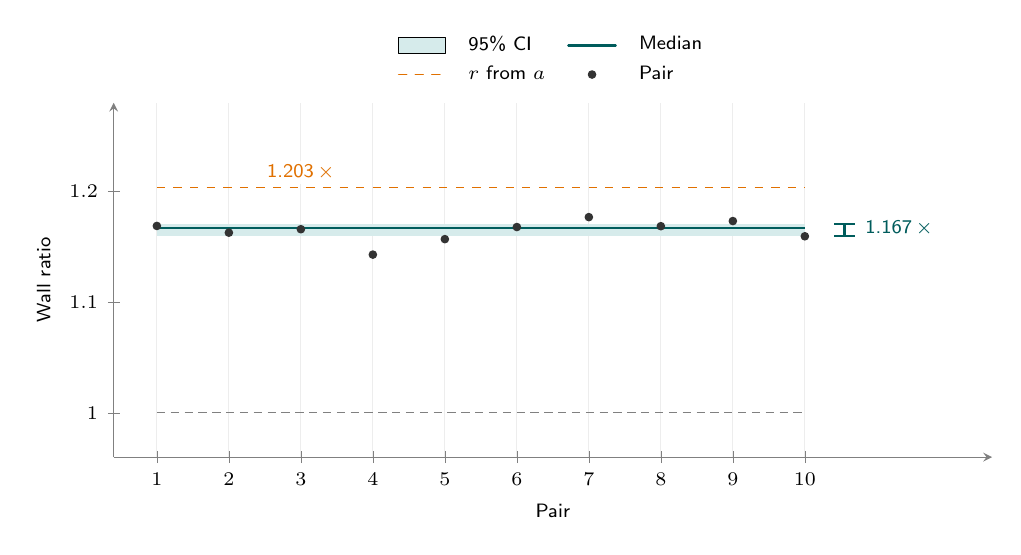
\begin{tikzpicture}
\begin{axis}[
  acts,
  width=0.92\columnwidth,
  height=4.5cm,
  xmin=0.4, xmax=12.6,
  ymin=0.96, ymax=1.28,
  xlabel={Pair},
  ylabel={Wall ratio},
  xtick={1,2,3,4,5,6,7,8,9,10},
  ytick={1,1.1,1.2},
  legend style={at={(0.5,1.03)}, anchor=south, legend columns=2},
]
% source: snpeff_alternating_carc.json bootstrap ci95 [1.1594573,1.1705137] around median_r
\addlegendimage{area legend, fill=actstealfaint, draw=none}
\addlegendentry{95\% CI}
\fill[actstealfaint] (axis cs:1,1.1594573) rectangle (axis cs:10,1.1705137);
\addlegendimage{actsteal, line width=0.9pt, mark=none}
\addlegendentry{Median}
\draw[actsteal, line width=0.9pt] (axis cs:1,1.1668229) -- (axis cs:10,1.1668229);
\addlegendimage{actsorange, dashed, mark=none}
\addlegendentry{$r$ from $a$}
% source: snpeff_alternating_carc.json r_from_a_now=1.2032081
\draw[actsorange, dashed] (axis cs:1,1.2032081) -- (axis cs:10,1.2032081);
\node[actlab, anchor=south, text=actsorange, yshift=1pt] at (axis cs:3,1.2032081) {1.203\,$\times$};
\draw[actsrule, densely dashed] (axis cs:1,1) -- (axis cs:10,1);
% source: snpeff_alternating_carc.json pairs.r
\addlegendimage{only marks, mark=*, mark size=1.35pt, draw=actsink, fill=actsink}
\addlegendentry{Pair}
\addplot[only marks, mark=*, mark size=1.35pt, actsink, forget plot] coordinates {(1,1.1687908) (2,1.16273) (3,1.1658284) (4,1.1429052) (5,1.1568851) (6,1.1678174) (7,1.1767678) (8,1.1685695) (9,1.1732101) (10,1.1594573)};
\draw[actsteal, line width=0.8pt] (axis cs:10.55,1.1594573) -- (axis cs:10.55,1.1705137);
\draw[actsteal, line width=0.8pt] (axis cs:10.41,1.1594573) -- (axis cs:10.69,1.1594573);
\draw[actsteal, line width=0.8pt] (axis cs:10.41,1.1705137) -- (axis cs:10.69,1.1705137);
\node[actlab, anchor=west, text=actsteal] at (axis cs:10.77,1.1668229) {1.167\,$\times$};
\end{axis}
\end{tikzpicture}
